% ARPEGOS:  Automatized Roleplaying-game Profile Extensible Generator Ontology based System %
% Author : Alejandro Muñoz Del Álamo %
% Copyright 2019 %

% Section 11.1: Objetivos alcanzados %
\section{Preparación}
\textit{\textbf{Nota informativa}}: En este manual no se va a explicar cómo funcionan las ontologías, ni cómo funciona \textit{Protégé}, 
sino cómo desarrollar ontologías para juegos de rol específicas para este proyecto. 

El primer paso para empezar a crear la nueva ontología de nuestro \textit{RPG} es abrir el editor. La primera pantalla que 
aparece es la siguiente.\medskip

\begin{figure}[H]
    \centering
    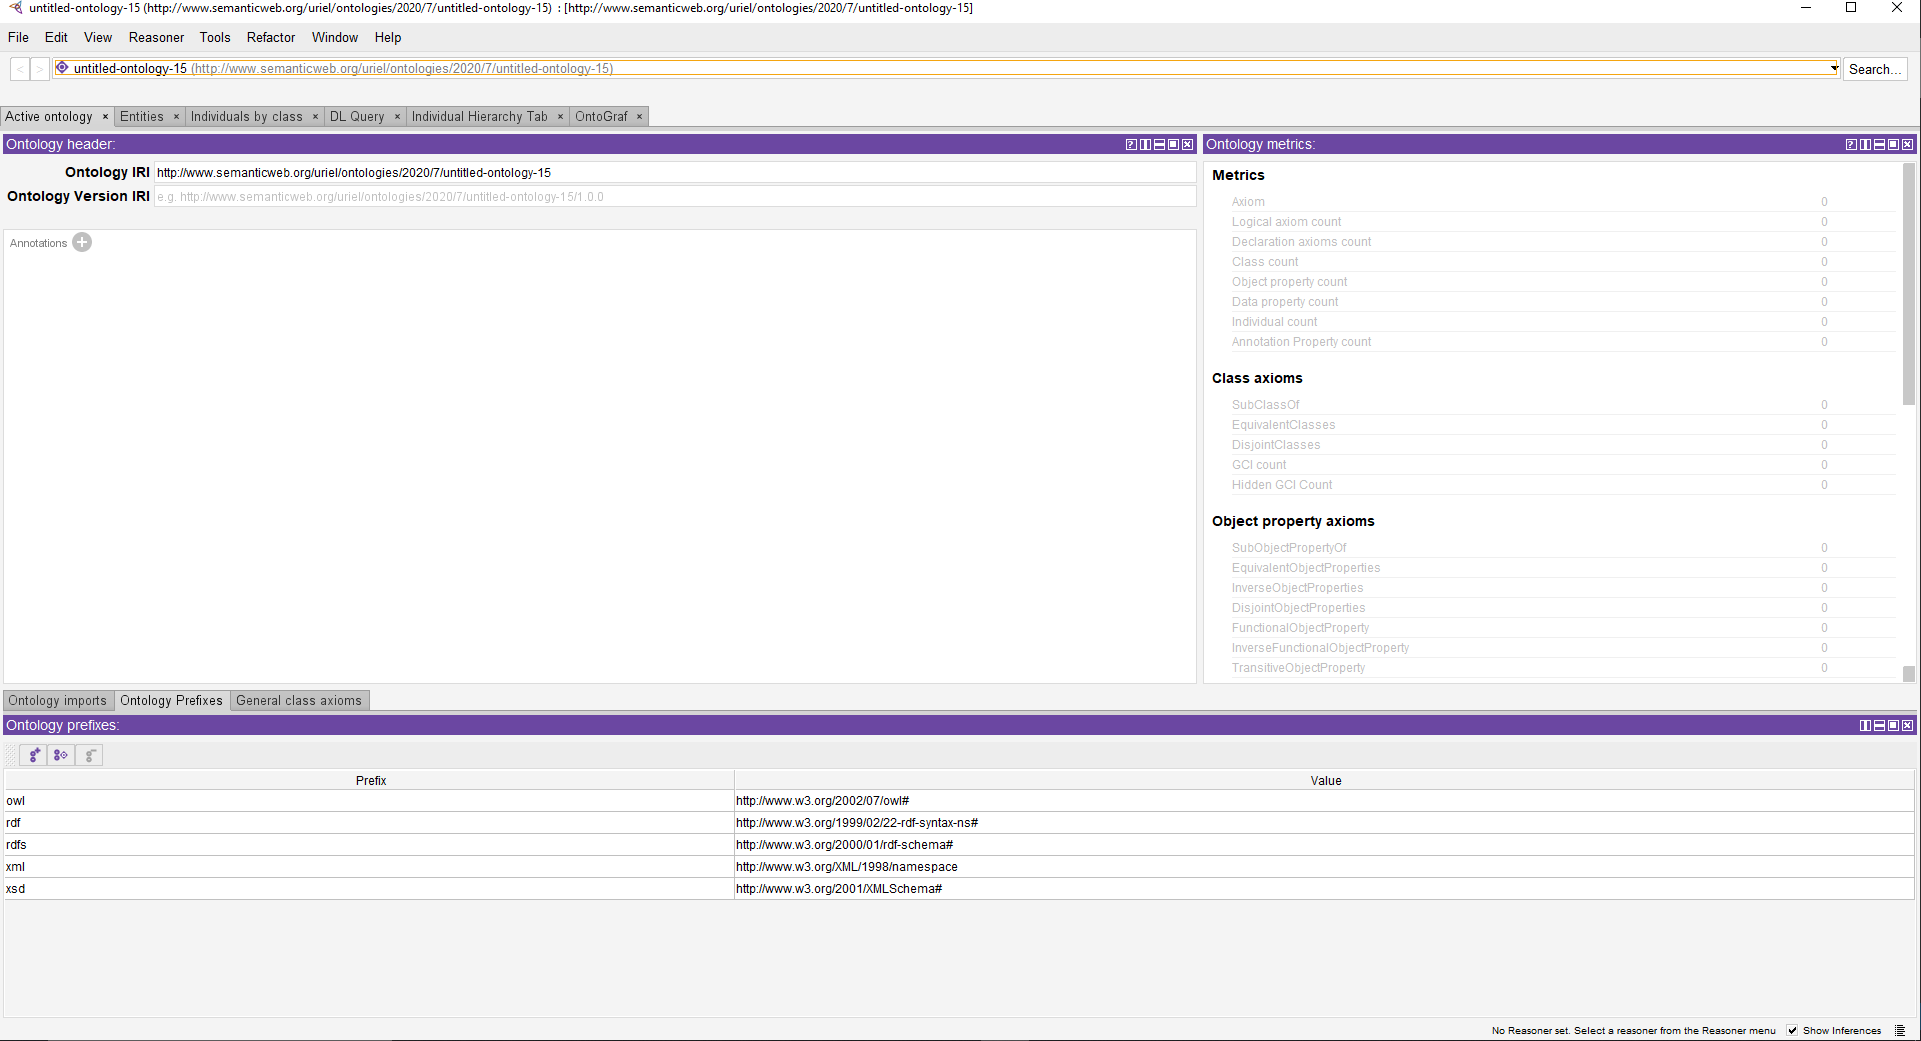
\includegraphics[scale=0.2]{Figures/Protege/Inicio_Protege.png}
    \caption{Pantalla inicial de \textit{Protégé}}
    \label{Inicio_protege}
\end{figure}

